\sectionframe{Current Development}
\section{Current}

\begin{frame}{Model in Continuous Time}
	\vspace{-1em}
	\begin{columns}
		\begin{column}{.3 \textwidth}
			\begin{align*}
				\overset{\cdot}{x} & = \lambda (x - 1) \quad & \text{if } & K_{F} = +1 \\
				\overset{\cdot}{x} & = \lambda x       \quad & \text{if } & K_{F} = 0  \\
				\overset{\cdot}{x} & = \lambda (x + 1) \quad & \text{if } & K_{F} = -1
			\end{align*}

			Switching at
			\begin{align*}
				V_{ref} \pm \chi_{c} \\
				V_{ref} \pm \chi_{0}
			\end{align*}
		\end{column}
		\begin{column}{.7 \textwidth}
			\begin{figure}
				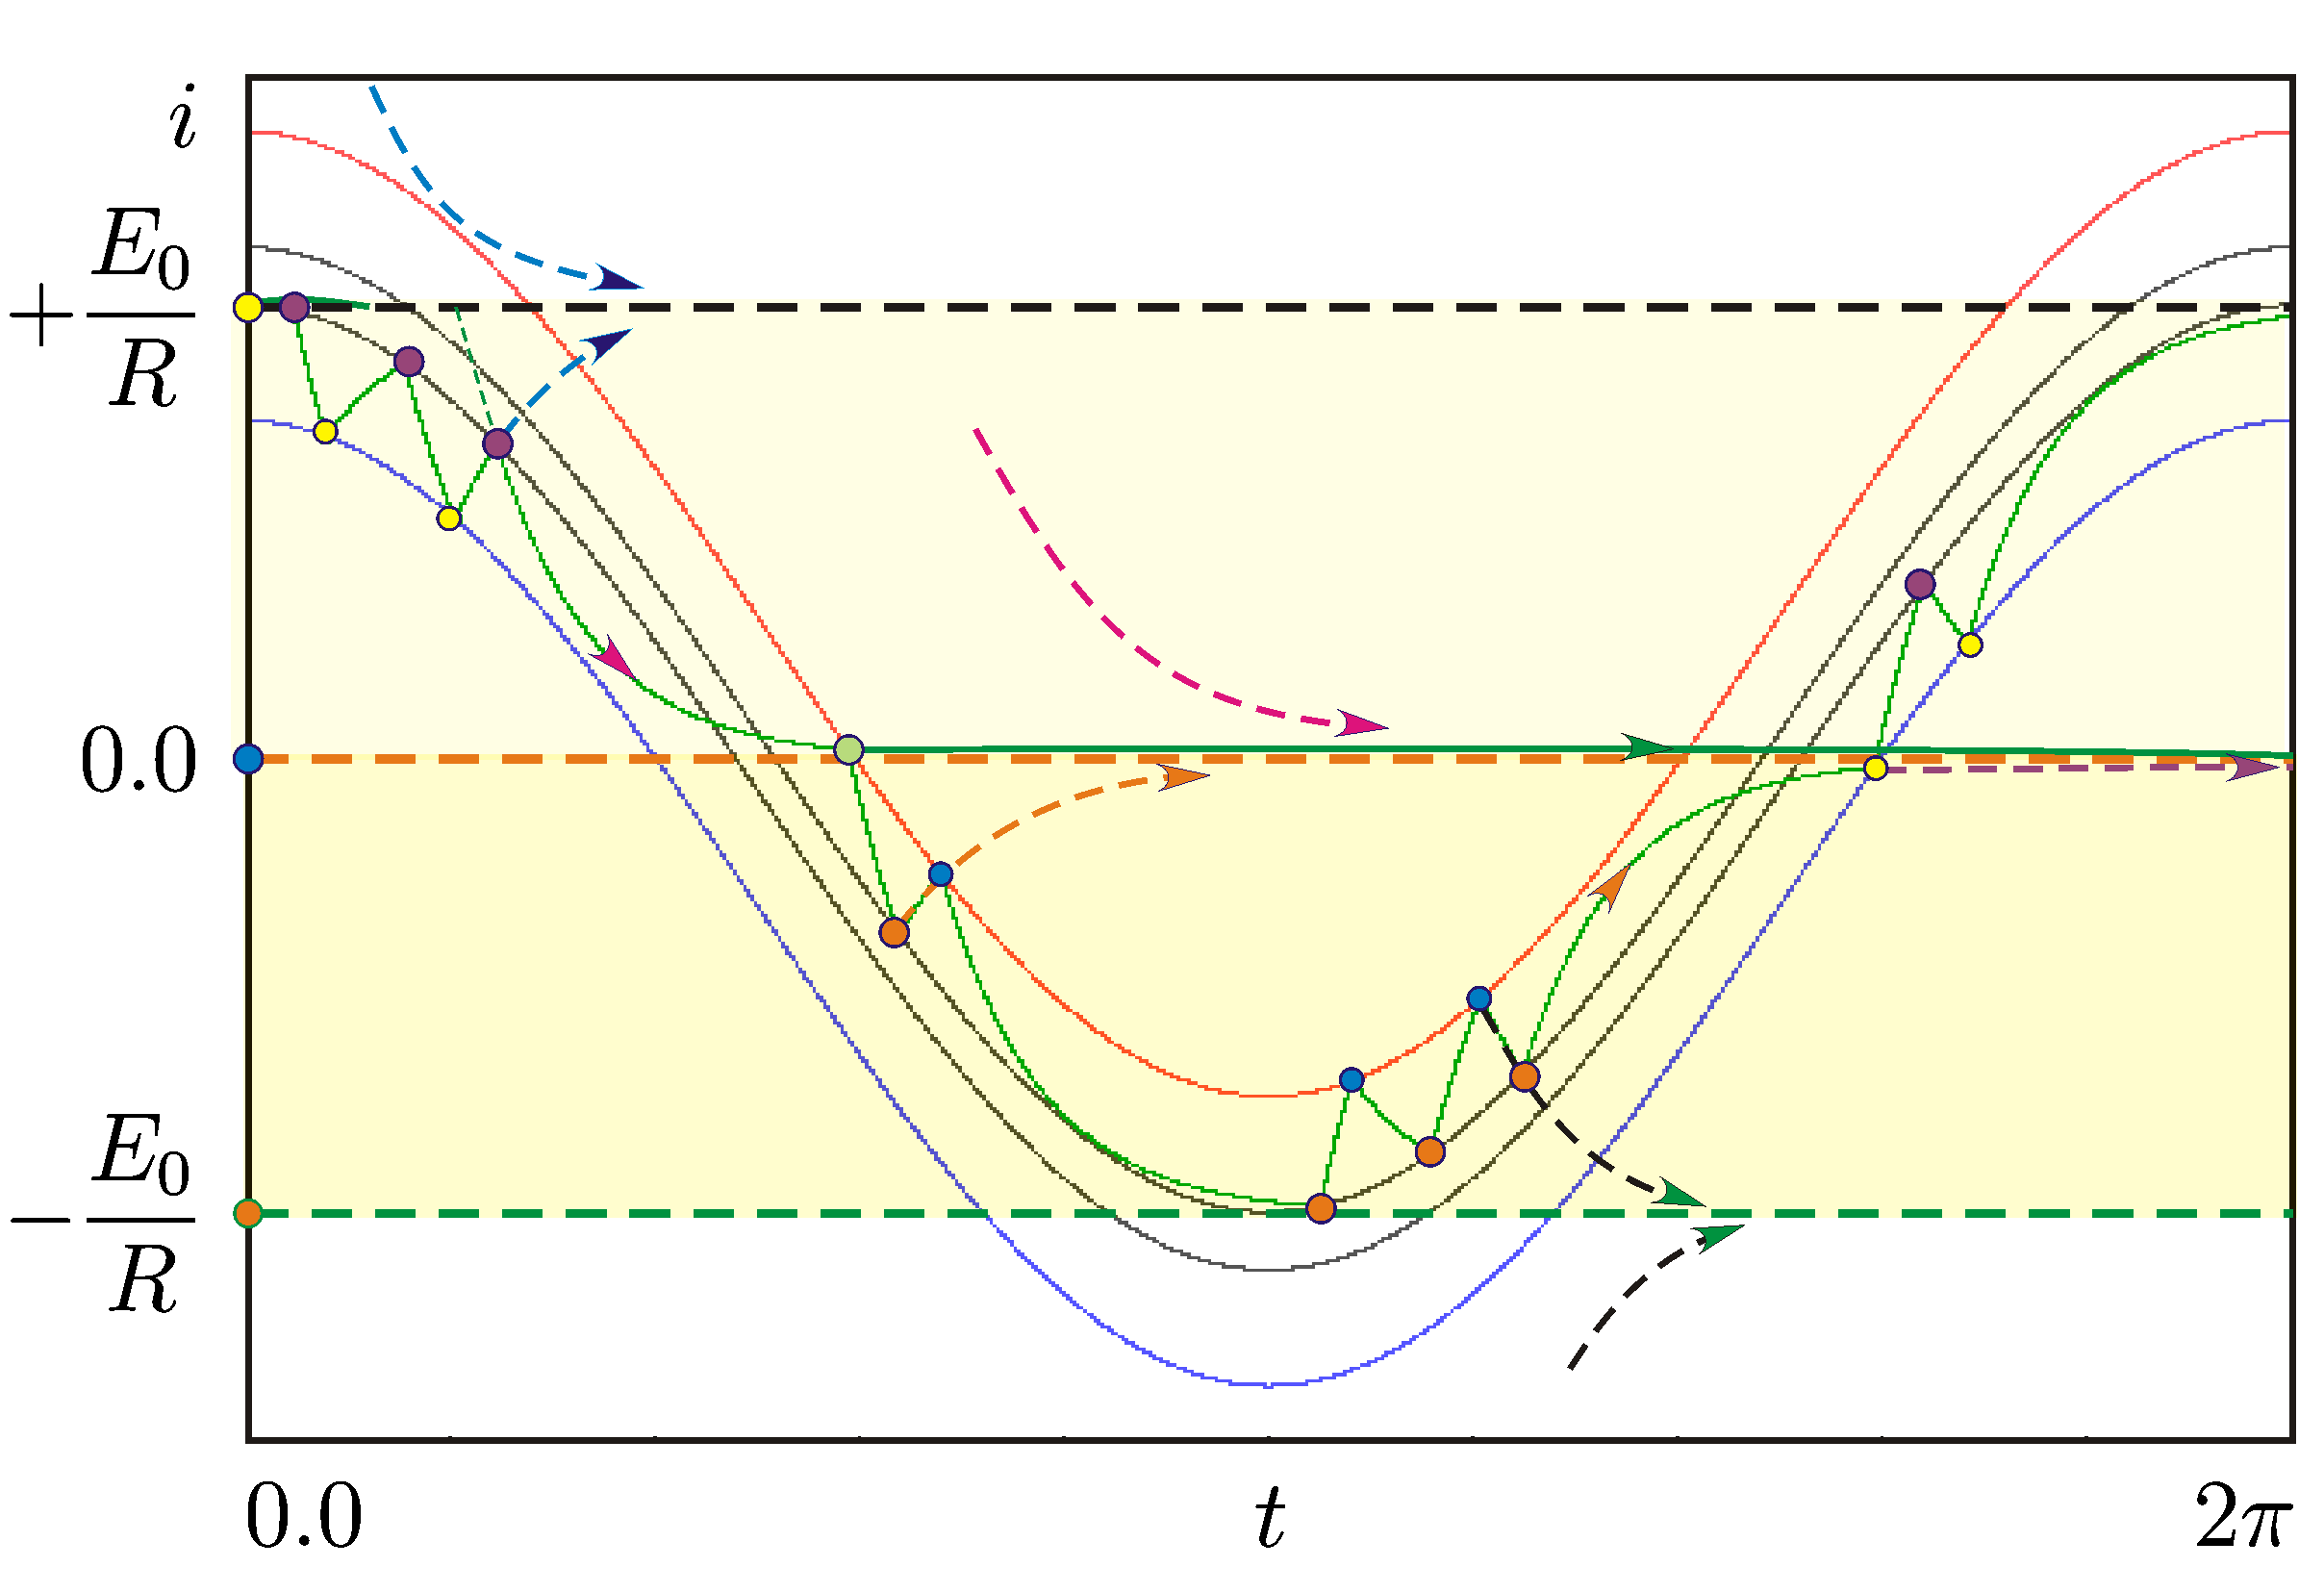
\includegraphics[width=0.7 \textwidth]{Figs/continuous_model.png}
			\end{figure}

			\flushright{[Zhusubaliyev]}
		\end{column}
	\end{columns}
\end{frame}

\begin{frame}{Model in Concrete Time}
	\vspace{-1em}
	\begin{columns}
		\begin{column}{.6 \textwidth}
			\begin{align*}
				(q \cos(\tau) - \chi_{c}) \cdot e^{z^{+}}                      = q \cos(\tau + z^{+}) - \chi_{0}            \\
				(q \cos(\tau + z^{+}) - \chi_{0} - 1) \cdot e^{z_{1}^{+}}      + 1  =                                \qquad \\
				q \cos(\tau + z^{+} + z_{1}^{+}) - \chi_{c}                                                                 \\\\
				(q \cos(\tau) - \chi_{c}) \cdot e^{z_{0}^{+}}                  = q \cos(\tau + z_{0}^{+}) + \chi_{0}        \\
				(q \cos(\tau + z_{0}^{+}) + \chi_{0} + 1) \cdot e^{z_{2}^{+}}  - 1  =                               \qquad  \\
				\hfill q \cos(\tau + z^{+} + z_{2}^{+}) + \chi_{c}
			\end{align*}
		\end{column}
		\begin{column}{.4 \textwidth}
			\begin{figure}
				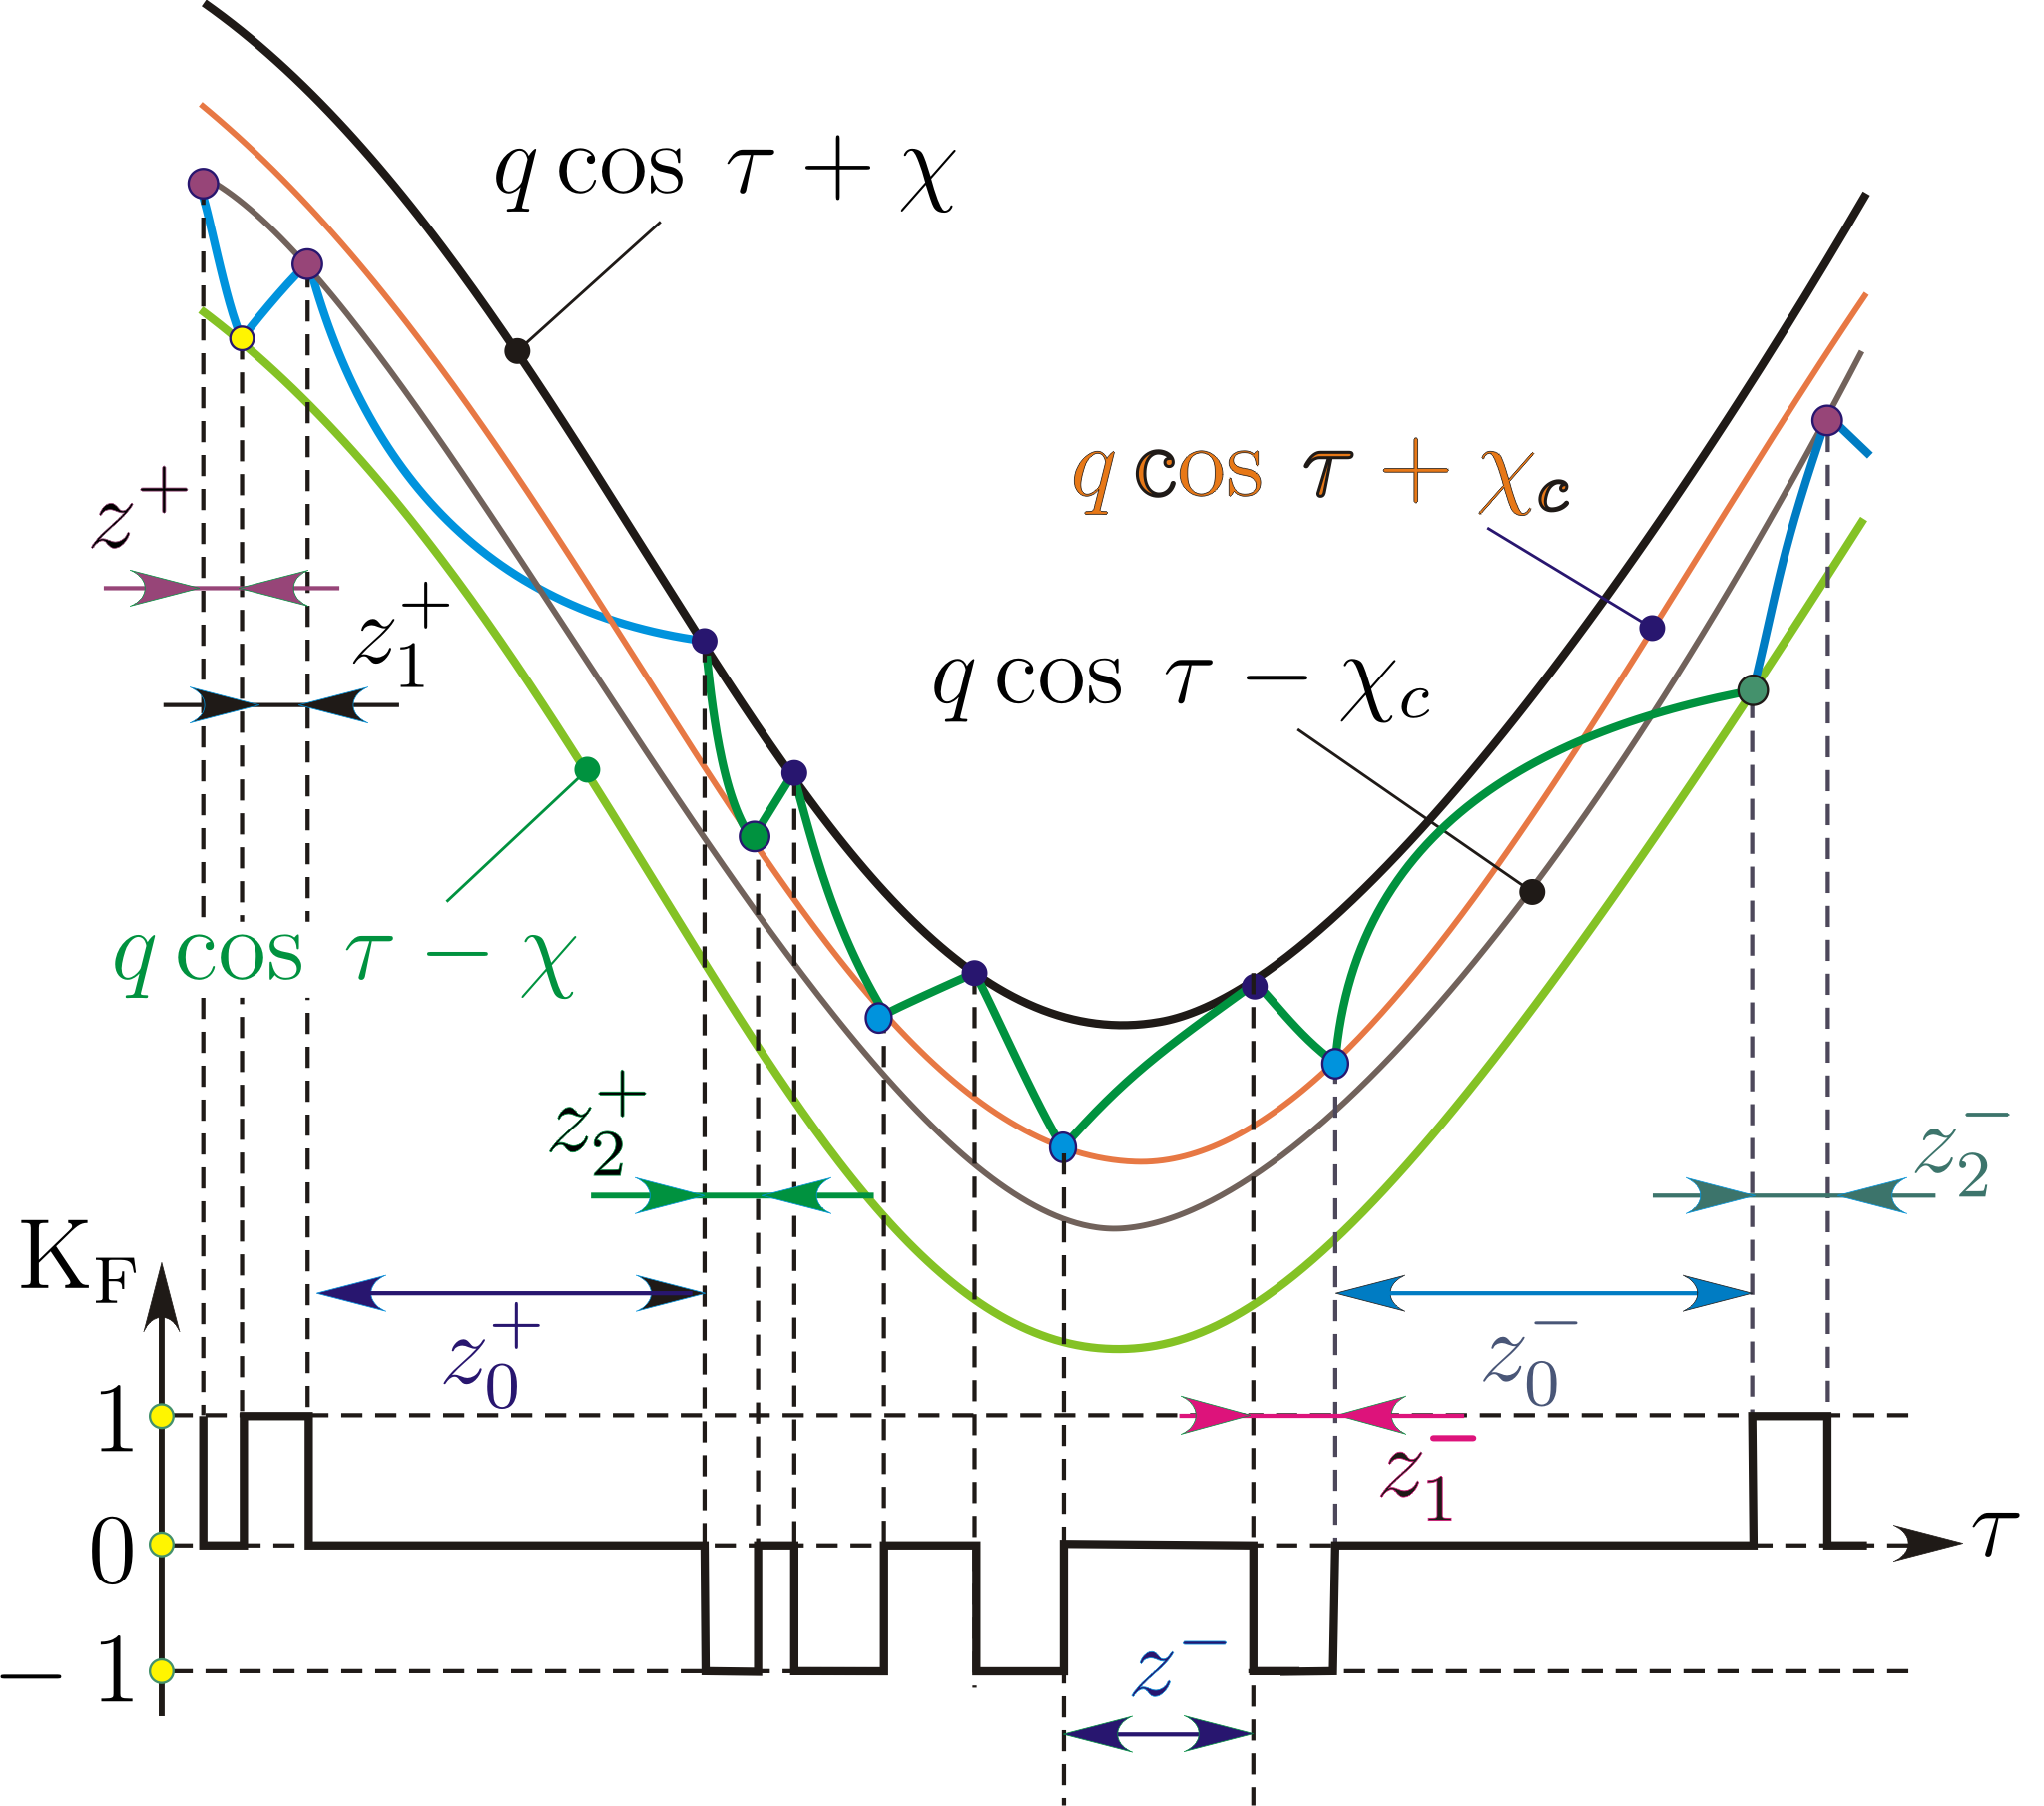
\includegraphics[width=0.9 \textwidth]{Figs/discrete_model_derivation.png}
			\end{figure}
		\end{column}
	\end{columns}

	\flushright{[Avrutin]}
\end{frame}

\begin{frame}{Model in Concrete Time}
	\vspace{-1em}
	\begin{columns}
		\begin{column}{.5 \textwidth}
			\begin{align*}
				\tau \mapsto  \tau + \begin{cases}
					                     z^{+} + z_{1}^{+}     & \text{if } z^{+} \leq z_{0}^{+} \\
					                     z_{0}^{+} + z_{2}^{+} & \text{if } z^{+} > z_{0}^{+}
				                     \end{cases}
			\end{align*}
			\vspace{1em}

			Repeat the whole process to get
			\begin{align*}
				z^{-}, z_{1}^{-}, z_{0}^{-}, \text{ and } z_{2}^{-}
			\end{align*}
		\end{column}
		\begin{column}{.5 \textwidth}
			\begin{figure}
				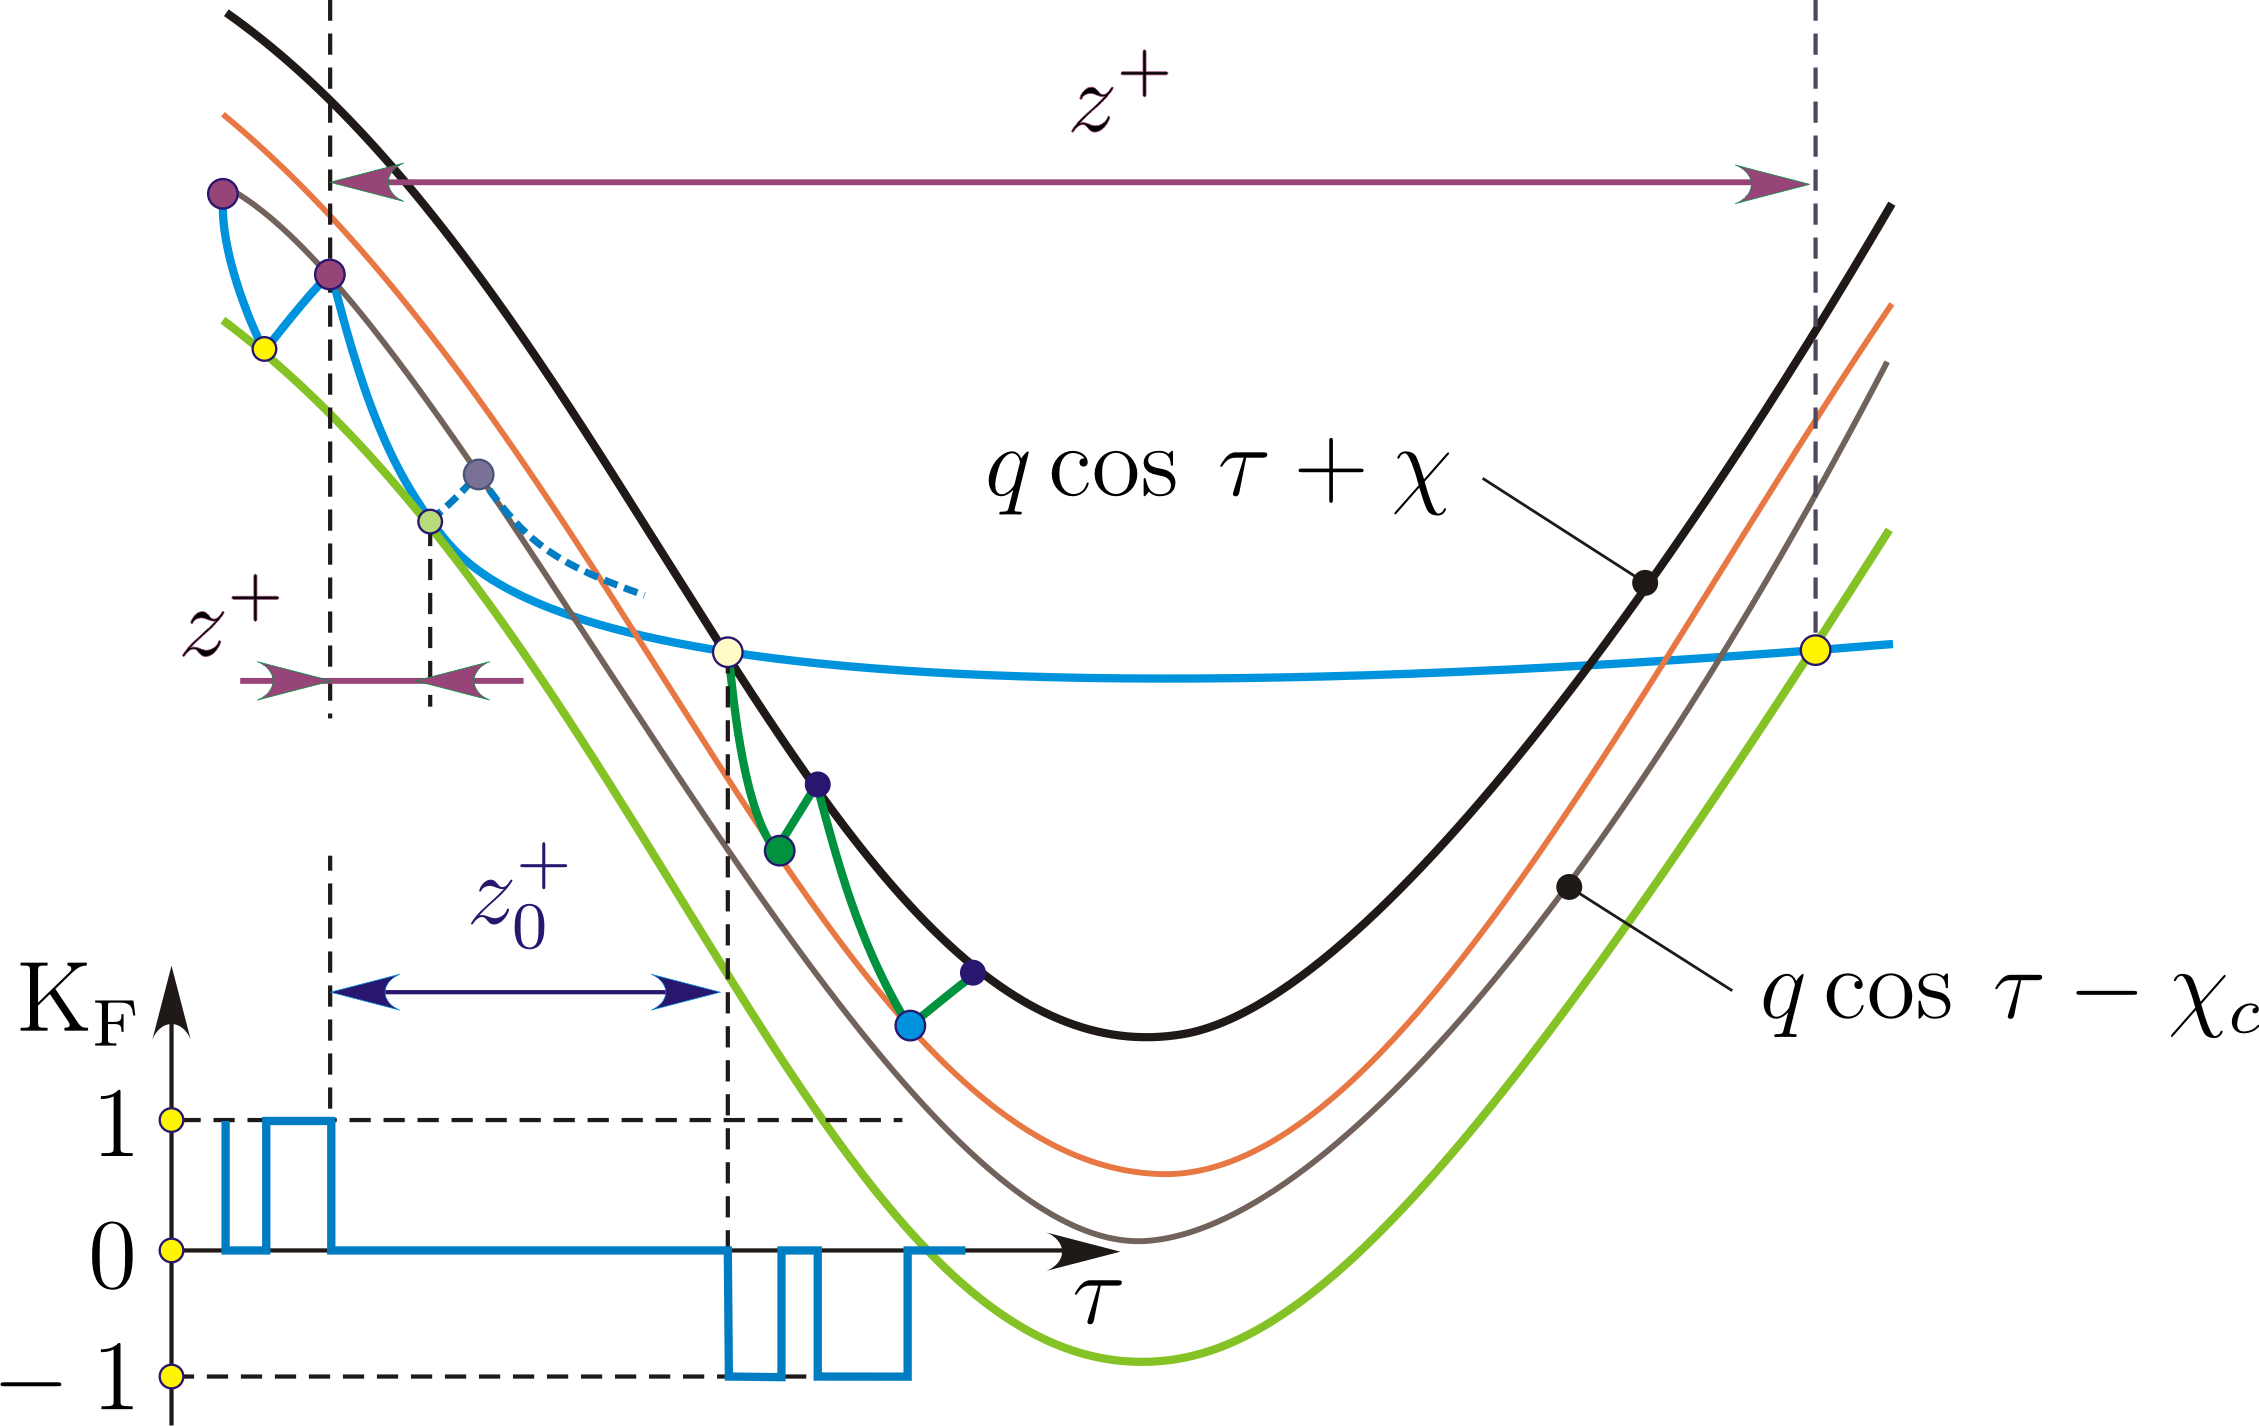
\includegraphics[width=1 \textwidth]{Figs/discrete_model_derivation_cases.png}
			\end{figure}
		\end{column}
	\end{columns}

	\flushright{[Avrutin]}
\end{frame}

\begin{frame}{Proof of Symmetry}
	TODO proof in paper

	\flushright{[Zhusubaliyev]}
\end{frame}

\begin{frame}{Proof of Symmetry}
	\begin{figure}
		\only<1>{
			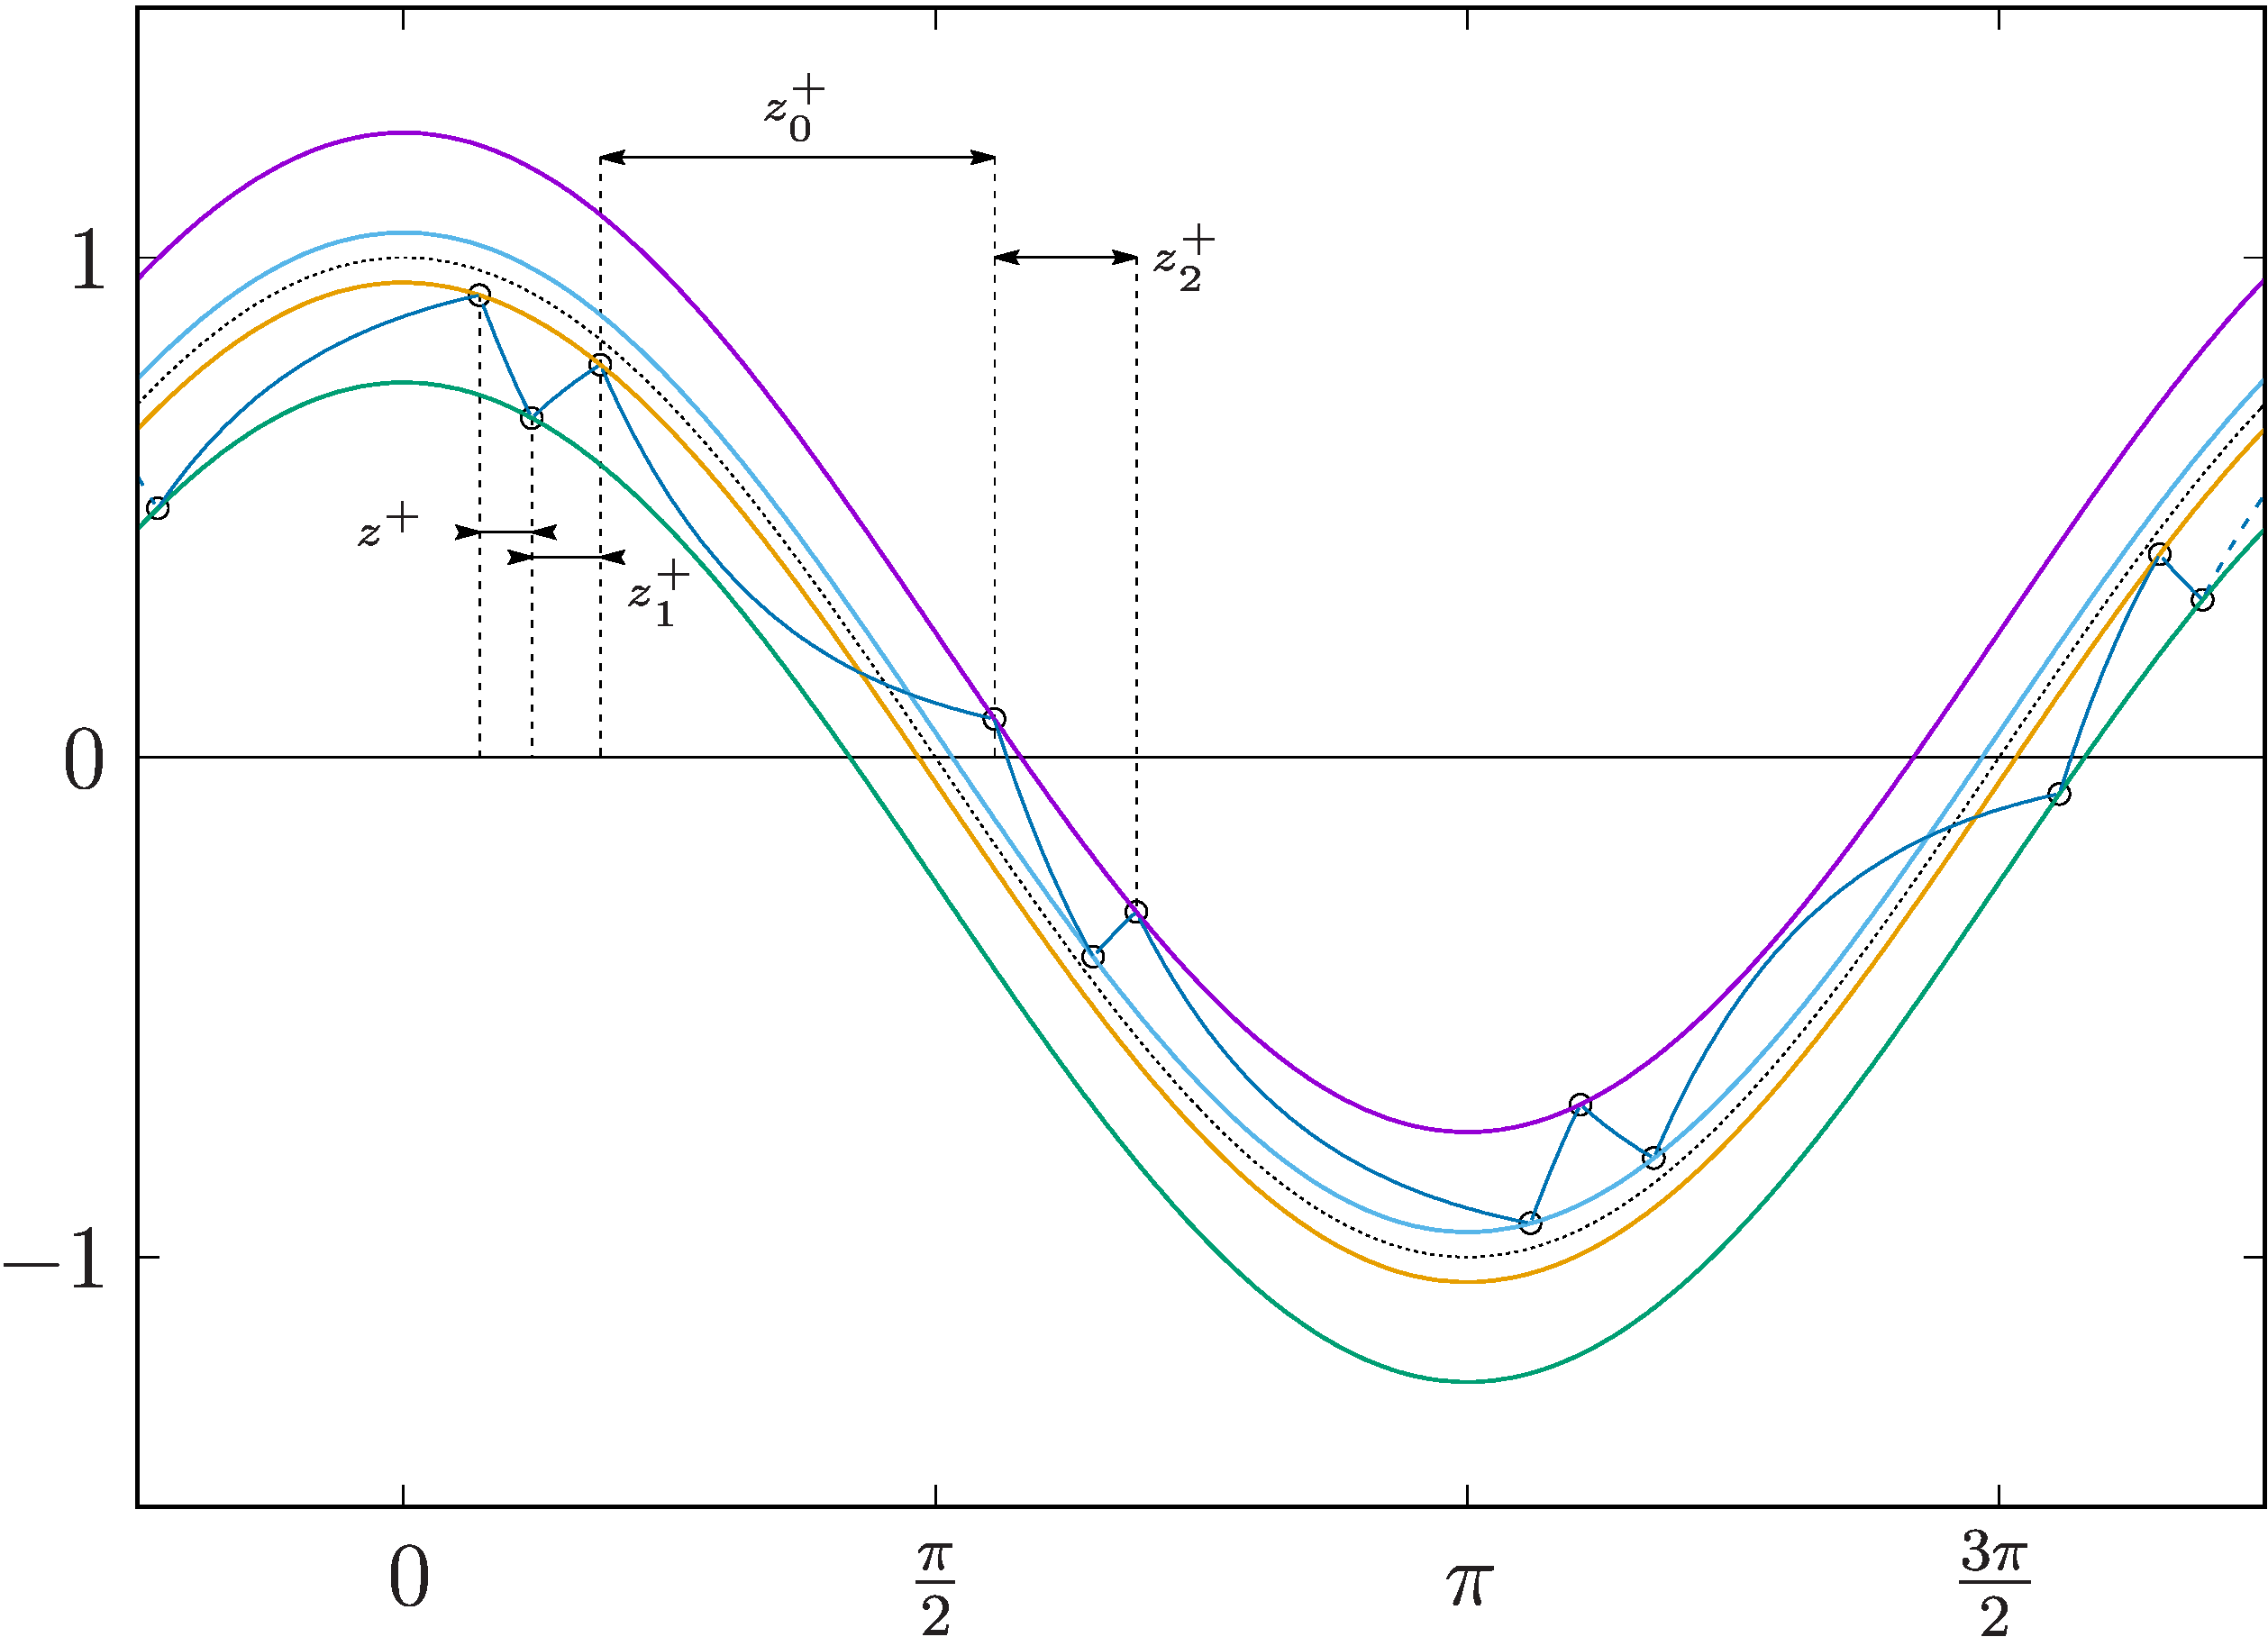
\includegraphics[height=0.8 \textheight]{Figs/full_model_full.png}
		}
		\only<2>{
			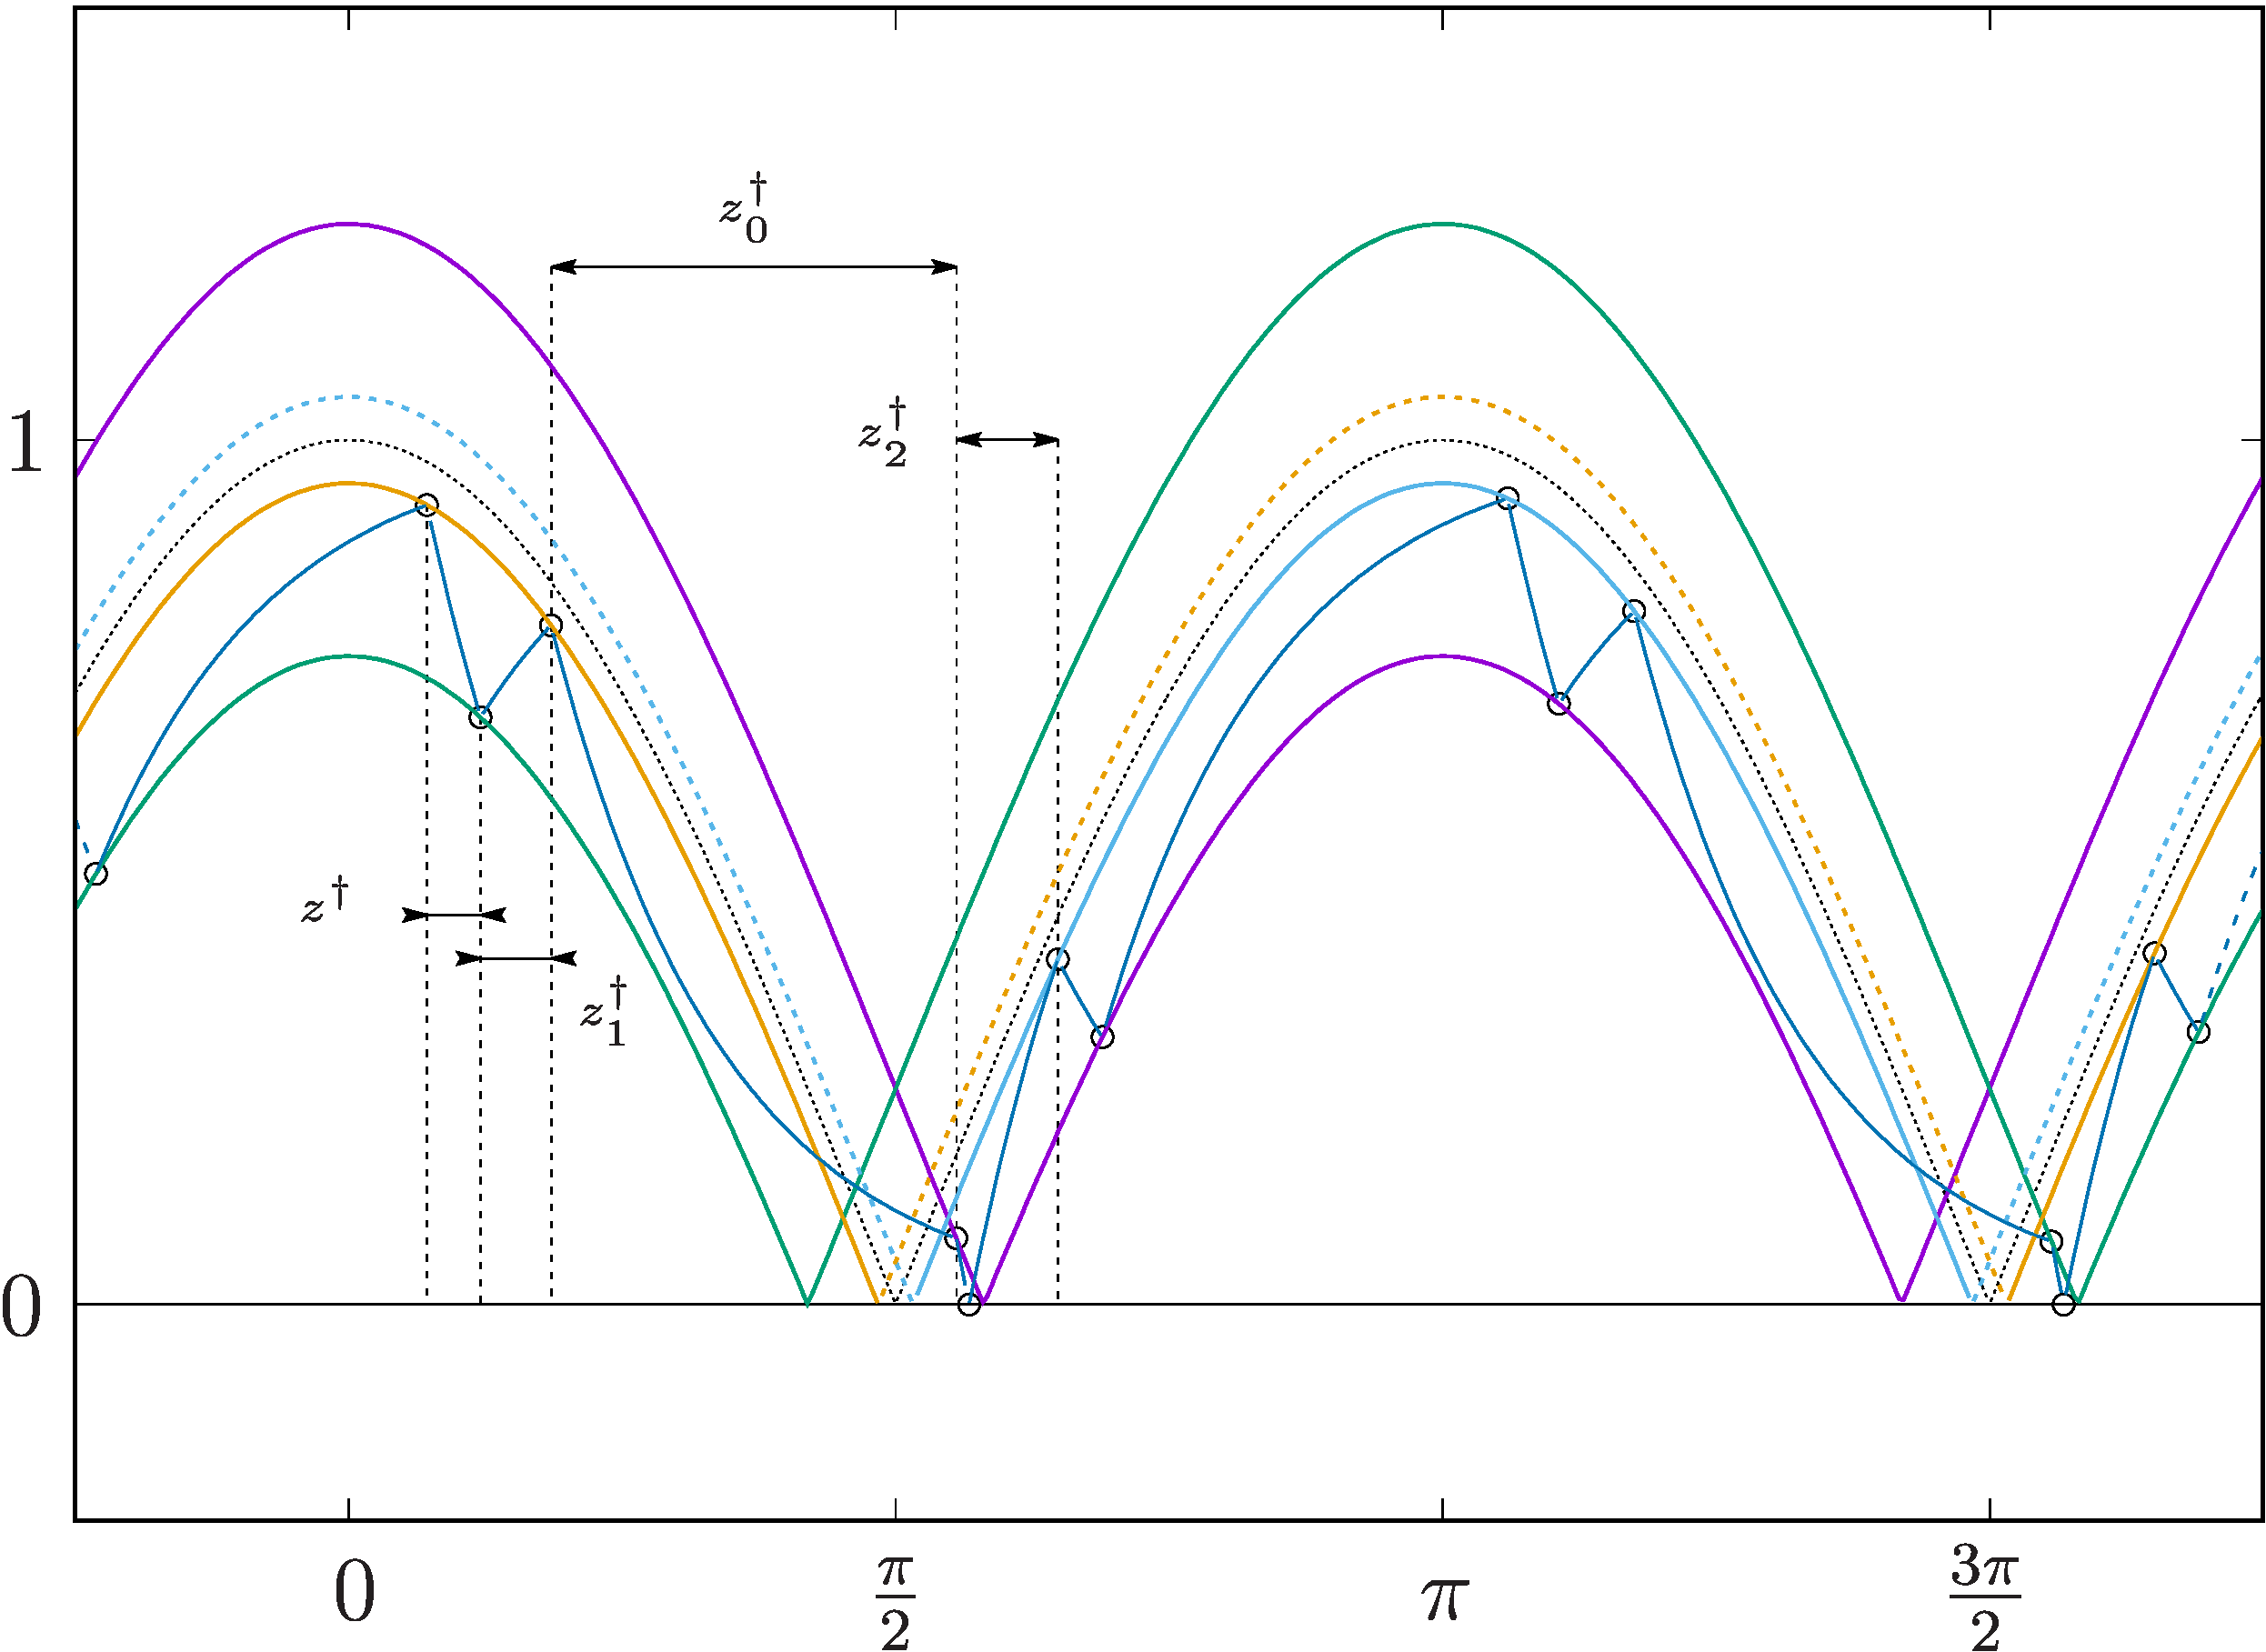
\includegraphics[height=0.8 \textheight]{Figs/absolute_model_full.png}
		}
		\only<3>{
			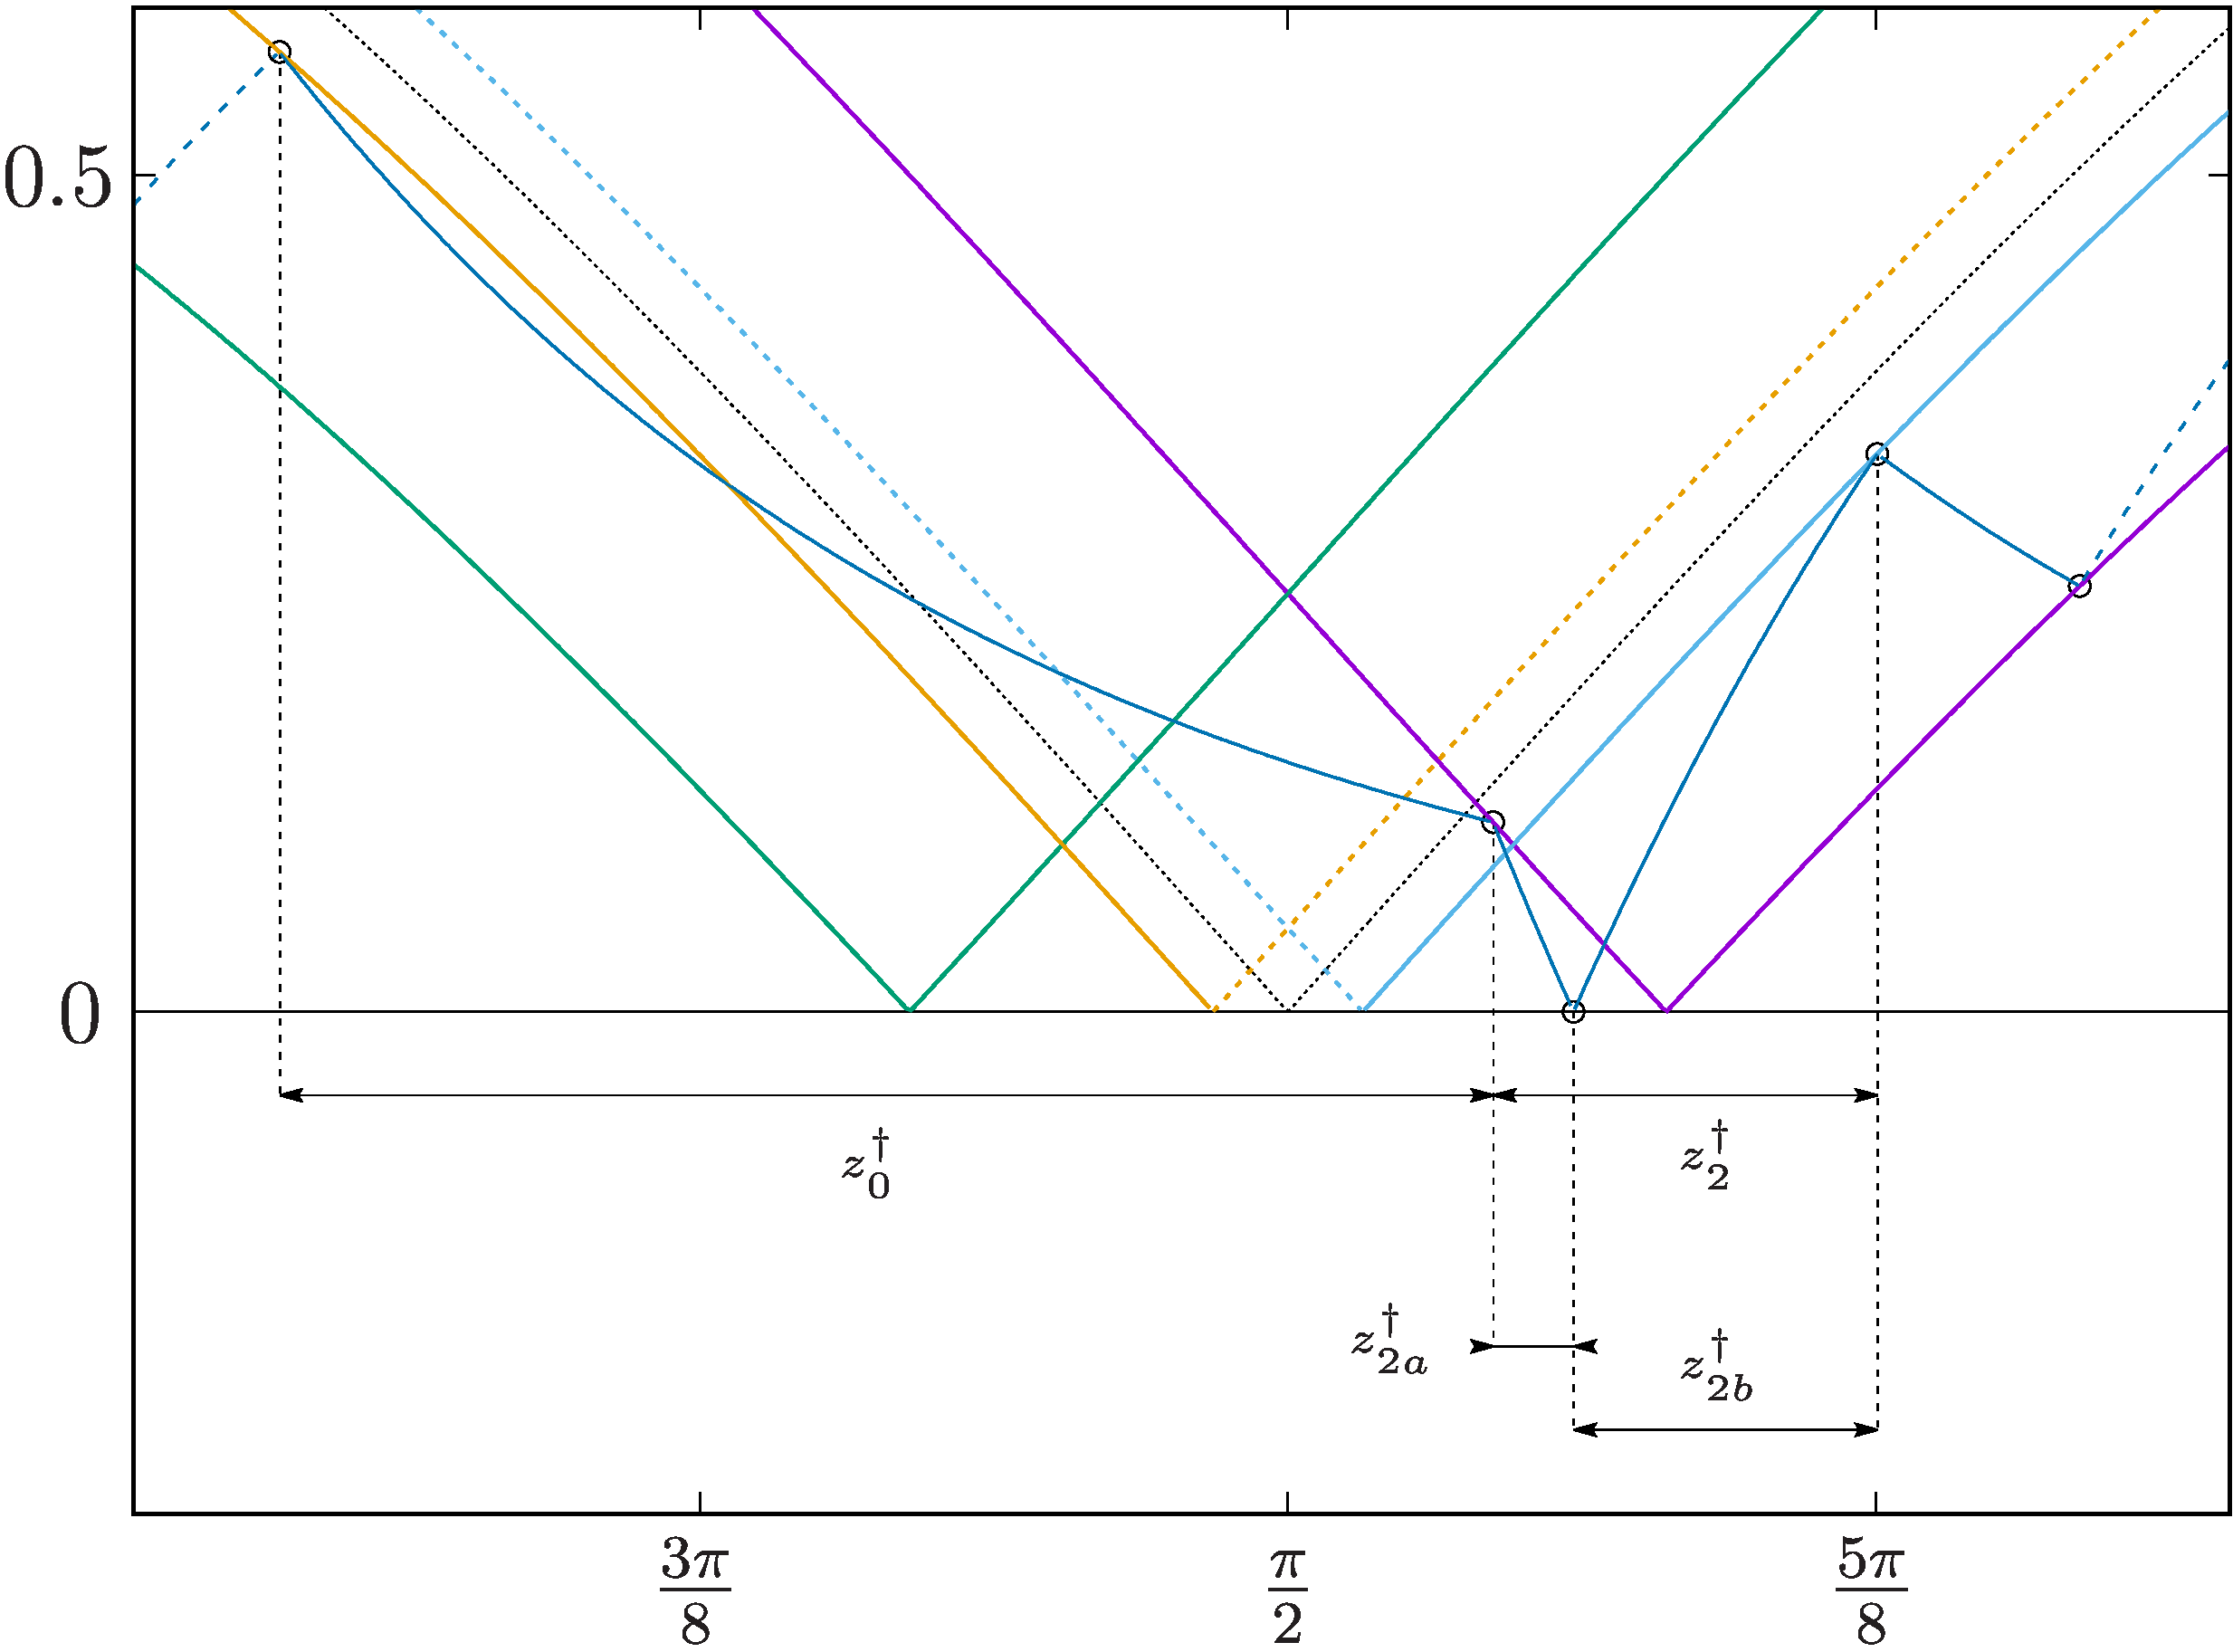
\includegraphics[height=0.8 \textheight]{Figs/absolute_model_zoomed.png}
		}
		\only<4>{
			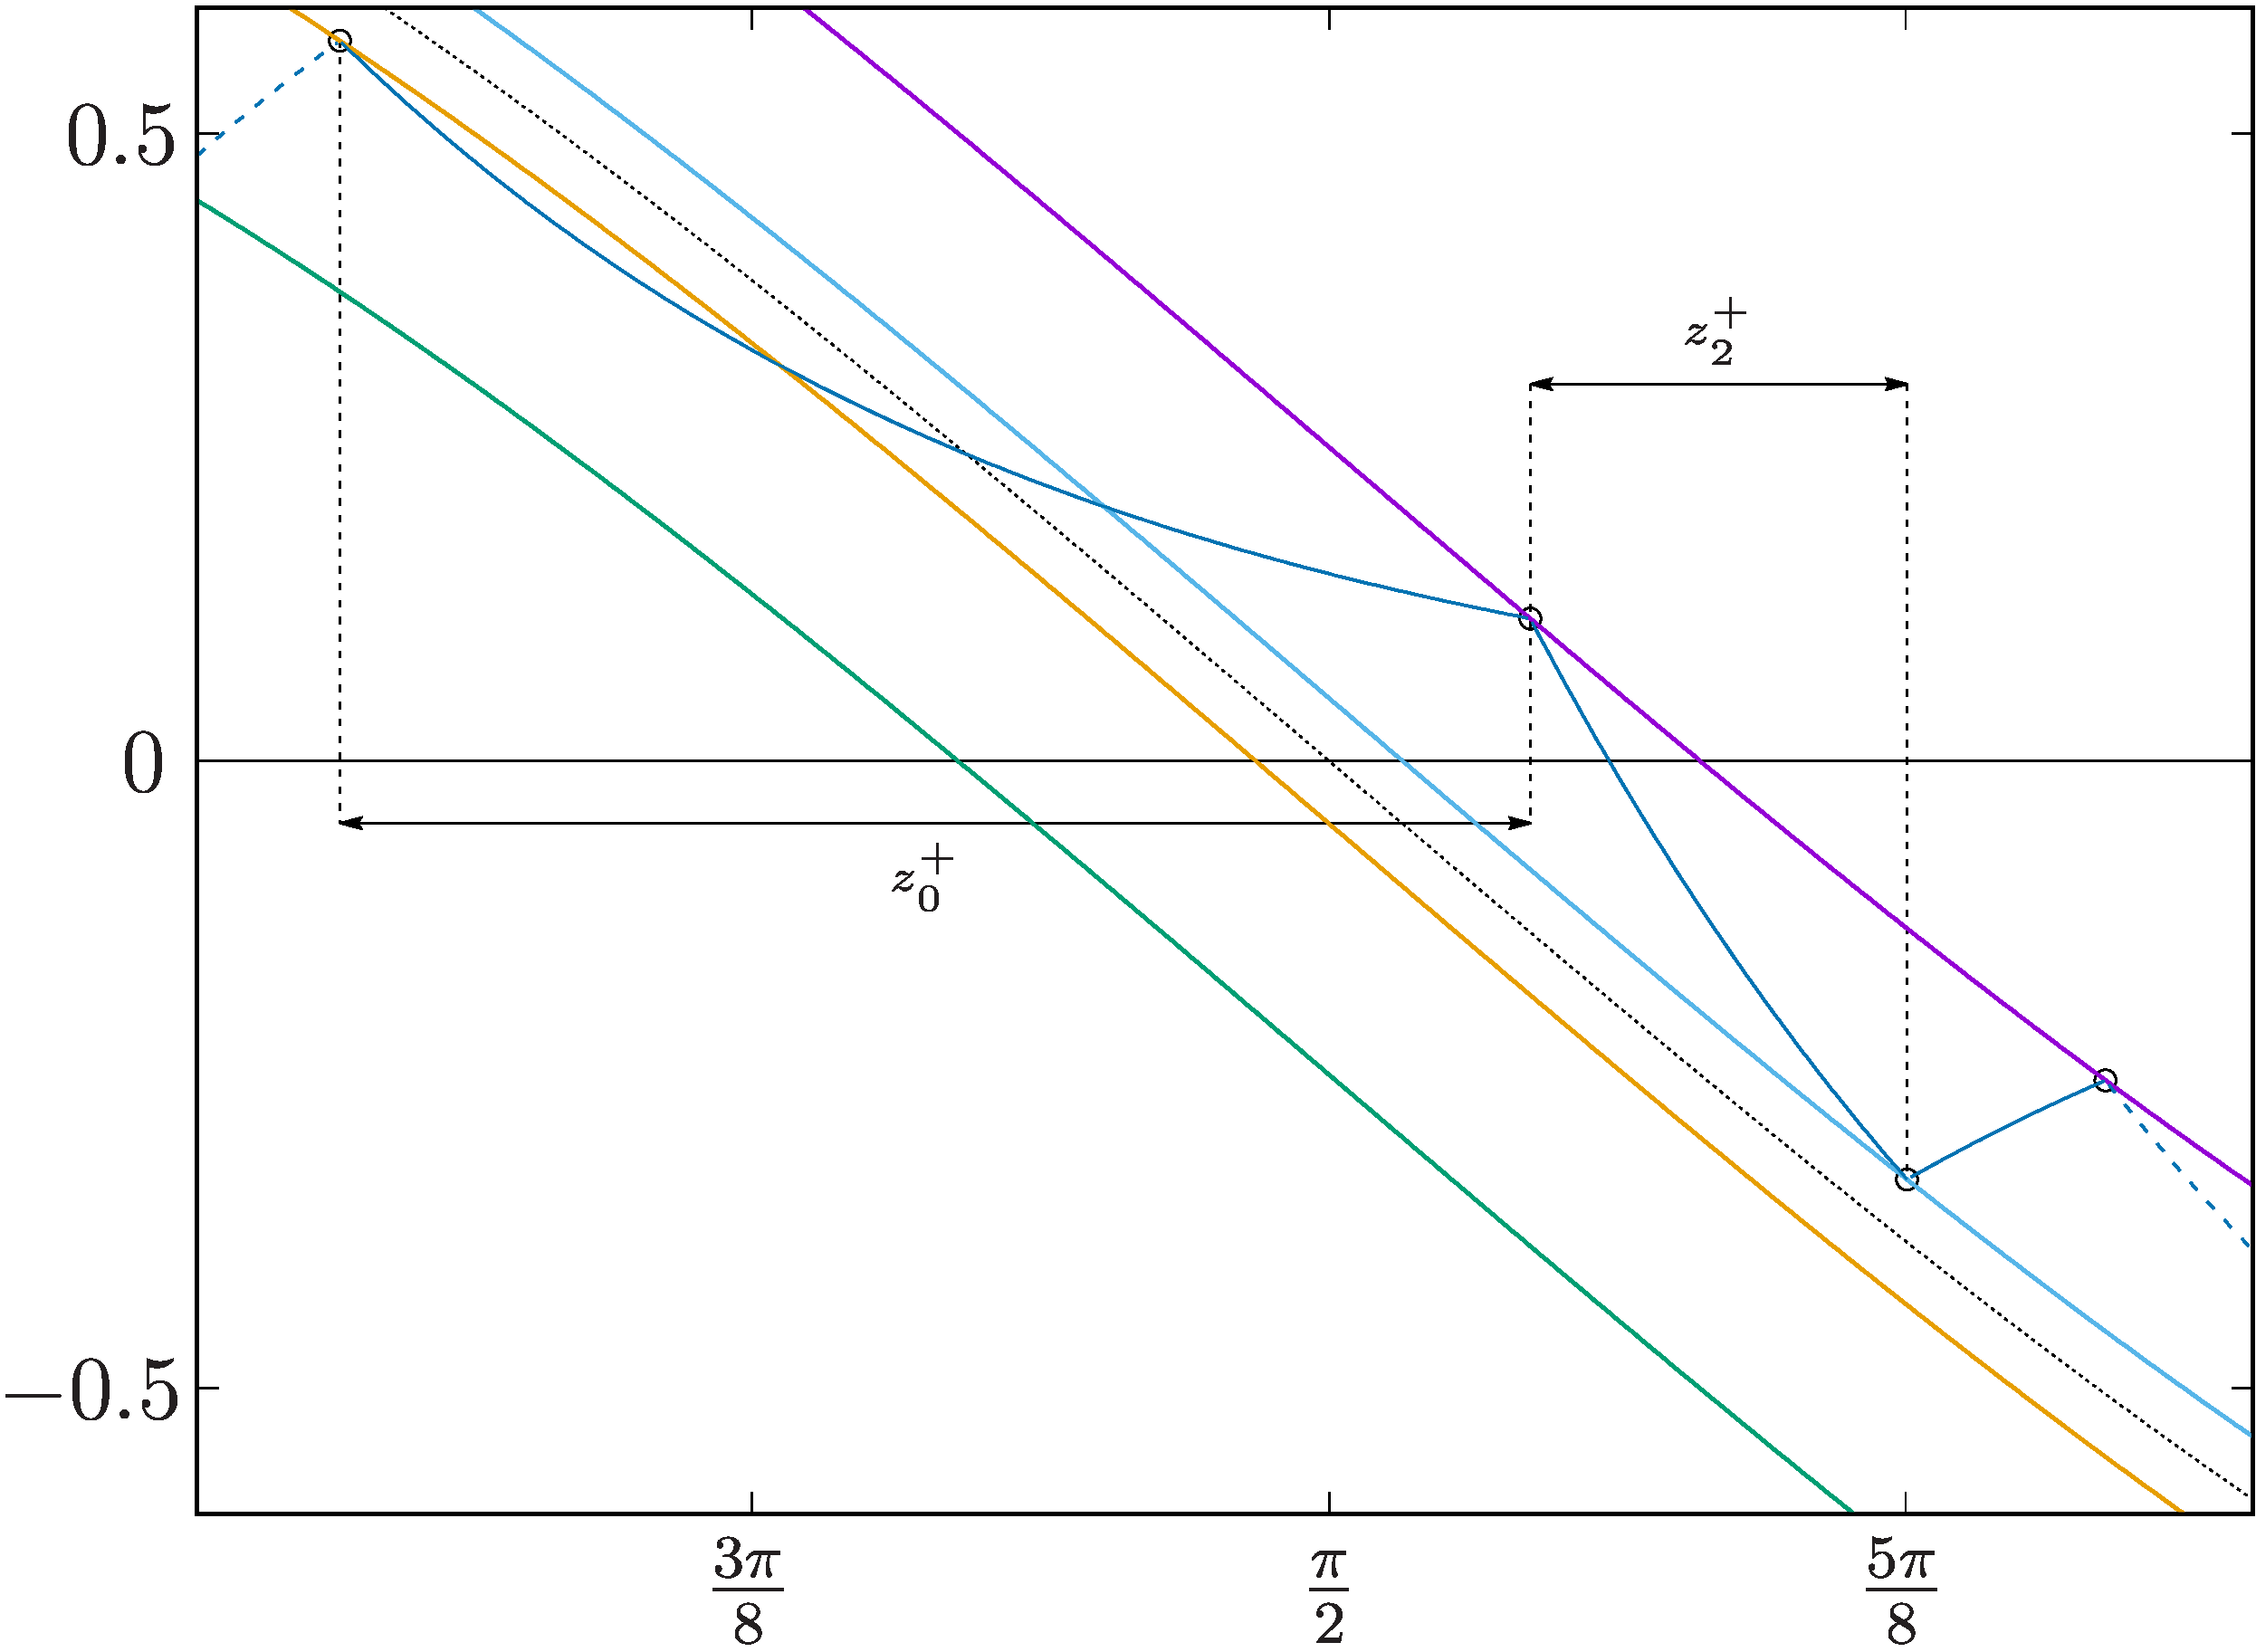
\includegraphics[height=0.8 \textheight]{Figs/full_model_zoomed.png}
		}
		\only<5>{
			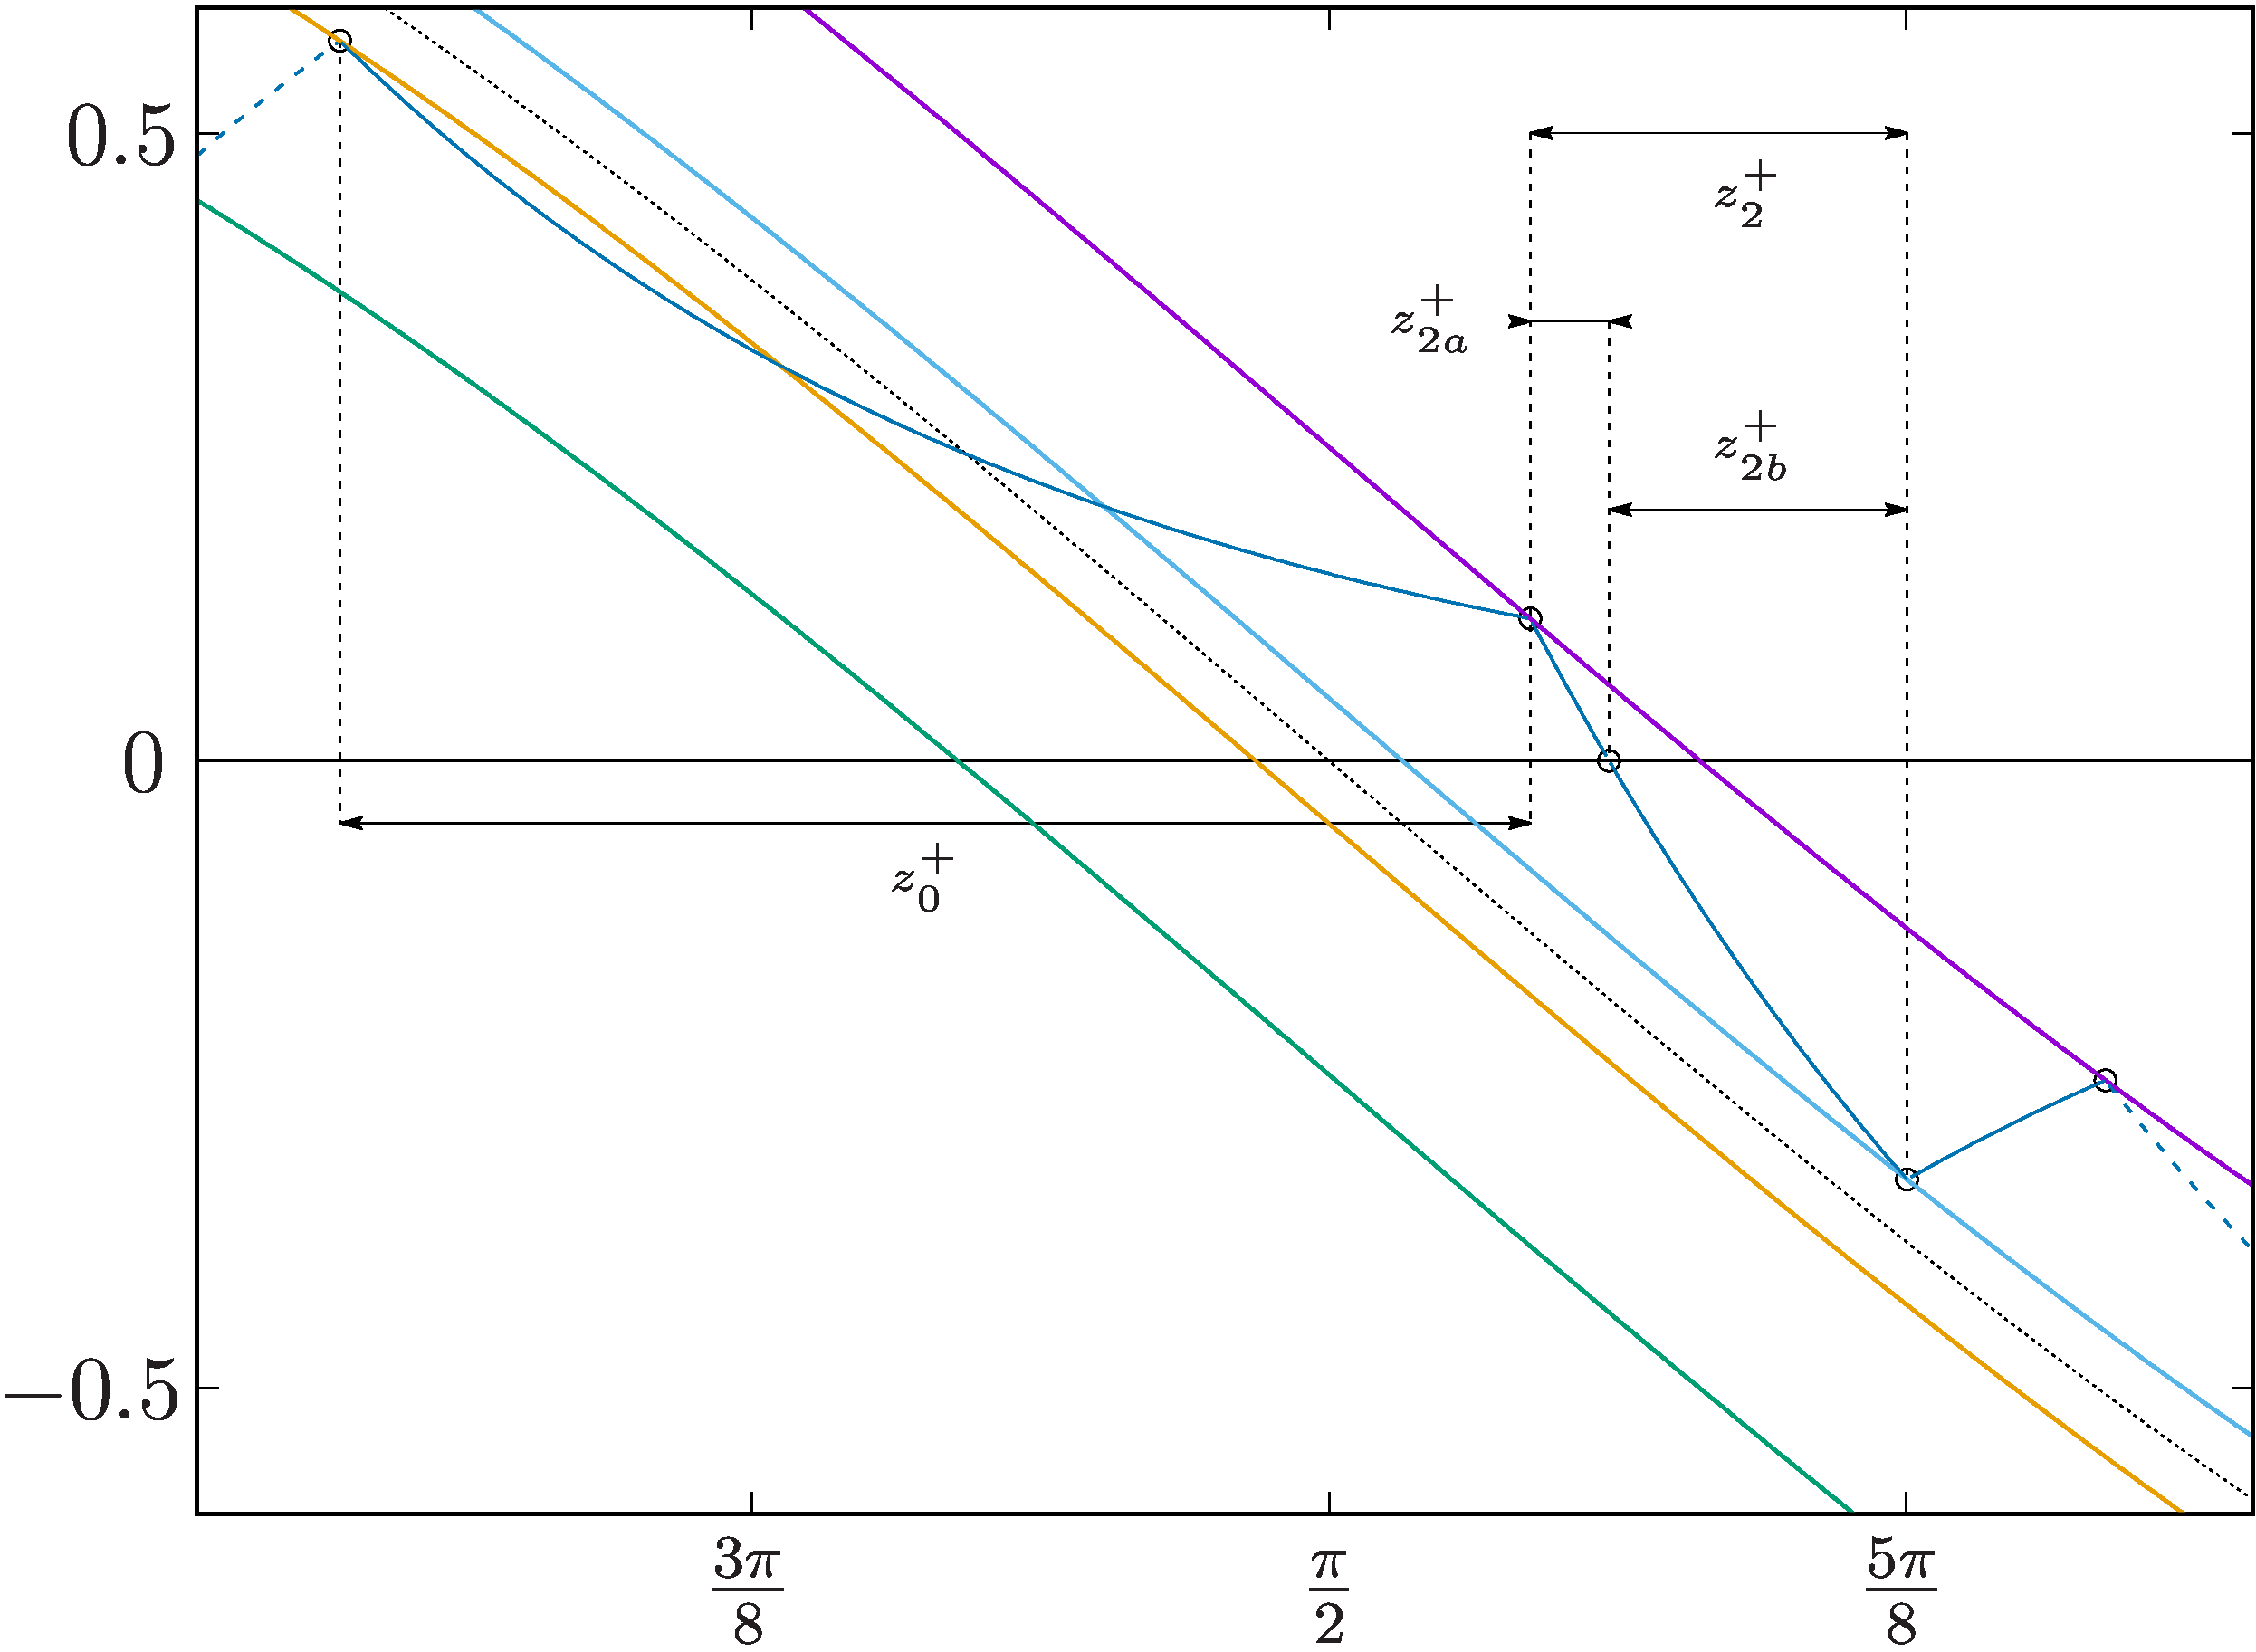
\includegraphics[height=0.8 \textheight]{Figs/full_virtual_model_zoomed.png}
		}
	\end{figure}
\end{frame}

\begin{frame}{General Proof of Symmetry}

\end{frame}


%%% Local Variables:
%%% TeX-master: "../Vortrag_Frauenhofer_Weik"
%%% End:
